\chapter{Povezivanje razvojnog sustava s bazom podataka}

Za programiranje modula ESP32-C3 korišten je \textit{ESP-IDF}, službeni radni okvir za razvoj softvera na ESP mikrokontrolerima.

\cite{firebase_esp32}

\section{Modeliranje stvarnog IoT sustava}

Na slici \ref{fig:stvarni_slucaj} nalazi se blok shema pokaznog IoT sustava. Za razvoj mobilne aplikacije korišten je radni okvir \textit{Flutter}, koji omogućava paralelan razvoj aplikacija na Android i iOS uređajima. 

Mobilna aplikacija dohvaća podatke iz baze podataka te ih prikazuje na grafu. 

\begin{figure}[ht]
	\centering
	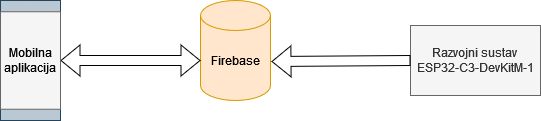
\includegraphics[scale=0.6]{imgs/stvarni_slucaj}
	\caption{Blok shema demo sustava}
	\label{fig:stvarni_slucaj}
\end{figure}

\eject